\documentclass[sigconf]{acmart}

\AtBeginDocument{%
  \providecommand\BibTeX{{Bib\TeX}}}

% TODO: Replace these fields with the values provided by the forum or ACM rights form.
\setcopyright{acmlicensed}
\copyrightyear{2026}
\acmYear{2026}
\acmDOI{XXXXXXX.XXXXXXX}
\acmConference[free5GC WF '26]{free5GC World Forum}{2026}{TBD}
\acmISBN{978-1-4503-XXXX-X/2026/XX}

\usepackage{listings}
\usepackage{balance}
\graphicspath{{../img/}}

\lstset{
  basicstyle=\ttfamily\footnotesize,
  breaklines=true,
  columns=fullflexible,
  frame=single,
  keepspaces=true,
  showstringspaces=false
}

\begin{document}

\title[Intent-Driven Orchestration for 5G Slices]{Intent-Driven Orchestration System for 5G RAN and Core Network Slices}

\author{Fang-Kai Ting}
\email{qawl987.cs13@nycu.edu.tw}
\affiliation{%
  \institution{National Yang Ming Chiao Tung University, Department of Computer Science}
  \city{Hsinchu}
  \country{Taiwan}}

\author{Fuchun Joseph Lin}
\email{fjlin@nycu.edu.tw}
\affiliation{%
  \institution{National Yang Ming Chiao Tung University, Department of Computer Science}
  \city{Hsinchu}
  \country{Taiwan}}

\author{Jyh-Cheng Chen}
\email{jcc@ncyu.edu.tw}
\affiliation{%
  \institution{National Yang Ming Chiao Tung University, Department of Computer Science}
  \city{Hsinchu}
  \country{Taiwan}}

\author{Chien Chen}
\email{chienchen@cs.nycu.edu.tw}
\affiliation{%
  \institution{National Yang Ming Chiao Tung University, Department of Computer Science}
  \city{Hsinchu}
  \country{Taiwan}}

\renewcommand{\shortauthors}{Ting and Chen}

\begin{abstract}
Network slicing requires coordinated control across the radio access network (RAN), the 5G core, and the cloud-native infrastructure that hosts network functions. Existing open-source 5G deployments expose these controls through heterogeneous and low-level interfaces, making it difficult to express service objectives as a single end-to-end policy. This paper presents an intent-driven orchestration system for free5GC and OCUDU. It models intents as Kubernetes custom resources, maps expectations to 5QI, S-NSSAI, PRB ratio, and scheduling priority, and applies them through a hybrid southbound design. We design and implement the OCUDU Operator, which is not supplied by Nephio or OCUDU, to realize RAN resources, while the official Nephio free5GC Operator manages core network-function lifecycles and a direct core path configures subscriber and QoS state. A Golang/Kubebuilder prototype demonstrates eMBB and URLLC slices over emulated UEs. Experiments show consistent configuration materialization and traffic differentiation. Management-plane latency is about 30 seconds, dominated by GitOps synchronization, while domain reconciliation completes within a fraction of a second.

\end{abstract}

\begin{CCSXML}
<ccs2012>
 <concept>
  <concept_id>10003033.10003099.10003102</concept_id>
  <concept_desc>Networks~Network management</concept_desc>
  <concept_significance>500</concept_significance>
 </concept>
 <concept>
  <concept_id>10003033.10003099.10003100</concept_id>
  <concept_desc>Networks~Cloud computing</concept_desc>
  <concept_significance>300</concept_significance>
 </concept>
 <concept>
  <concept_id>10003033.10003099.10003104</concept_id>
  <concept_desc>Networks~Network performance analysis</concept_desc>
  <concept_significance>300</concept_significance>
 </concept>
</ccs2012>
\end{CCSXML}

\ccsdesc[500]{Networks~Network management}
\ccsdesc[300]{Networks~Cloud computing}
\ccsdesc[300]{Networks~Network performance analysis}

\keywords{5G, network slicing, intent-driven management, free5GC, OCUDU, Nephio, Kubernetes, GitOps}

\maketitle

\section{Introduction}
\label{sec:introduction}

Network slicing is a central mechanism for supporting diverse service requirements in 5G and emerging 6G systems. A slice may be optimized for enhanced mobile broadband (eMBB), ultra-reliable low-latency communication (URLLC), massive IoT, or an operator-defined service class. In practice, however, a slice is not configured at a single point. The radio access network (RAN) must allocate radio resources and scheduling priority, the core network must bind subscribers and PDU sessions to QoS flows, and the cloud-native infrastructure must deploy and update network functions. This cross-domain nature creates a persistent gap between service-level objectives and the low-level knobs exposed by individual systems.

Intent-driven management addresses this gap by allowing a consumer to state the desired outcome rather than the sequence of operations required to achieve it. 3GPP TS 28.312 defines intent as an outcome-oriented management construct and discusses the lifecycle of intent handling, including translation, fulfillment, reporting, and conflict handling~\cite{3gpp_ts28312}. O-RAN similarly introduces RAN automation functions such as rApps for policy and optimization~\cite{oran_oad_r005}. Yet an open-source, end-to-end implementation that connects high-level intents to both free5GC and OCUDU remains difficult because the relevant controls live across different configuration systems, APIs, and reconciliation loops.

This work builds an intent-driven orchestration system for open-source 5G network slices. The design uses Kubernetes as the intent interface and execution substrate. A consumer submits an \texttt{E2EQoSIntent} custom resource that describes slice expectations, such as \texttt{bandwidth: high}, \texttt{latency: ultra-low}, and \texttt{resourceShare: Full}. The orchestrator translates these expectations into domain parameters: 5QI and QFI for the 5G core, plus S-NSSAI, PRB policy ratios, and scheduling priority for the RAN. RAN changes are handled as declarative Nephio package mutations and realized by the OCUDU Operator. In the core domain, the official Nephio free5GC Operator reconciles network-function deployments, while subscriber registration and QoS parameters are applied through free5GC-facing configuration logic.

The contributions are:
\begin{itemize}
  \item We design a Kubernetes-native intent model, \texttt{E2EQoSIntent}, for describing multiple 5G slice objectives in one end-to-end resource.
  \item We implement a translation layer from service-level expectations to concrete free5GC and OCUDU parameters, including 5QI, QFI, S-NSSAI, PRB policy ratio, and priority.
  \item An OCUDU Operator provides hierarchical CRDs, cross-resource validation, configuration rendering, and RAN reconciliation.
  \item We integrate Nephio/GitOps and domain operators into RAN and core NSSMF paths, with direct free5GC configuration for dynamic subscriber and QoS state.
  \item We evaluate the prototype with eMBB and URLLC slices and report both data-plane differentiation and management-plane orchestration latency.
\end{itemize}

\section{Background and Motivation}
\label{sec:background}

\subsection{5G Slice Management}

3GPP describes a network slice instance as an end-to-end logical network composed of slice subnets across domains such as the core network, RAN, and transport network~\cite{3gpp_ts28530}. Management systems commonly decompose this responsibility into a network slice management function (NSMF) and domain-specific network slice subnet management functions (NSSMFs)~\cite{3gpp_ts28533}. This decomposition is useful, but it leaves the operator with the problem of mapping service objectives into domain-specific parameters.

For the core network, free5GC implements a 5G core following the service-based architecture of 3GPP Release 15~\cite{free5gc,3gpp_ts23501}. Relevant slice and QoS controls include S-NSSAI, subscriber data, session management, QoS flow identifiers, and 5QI. For the RAN, OCUDU exposes practical controls for slice-aware scheduling through S-NSSAI-specific parameters, including PRB policy ratios and priority~\cite{ocudu,ocudu_oran_gnb_doc}. The challenge is not the absence of knobs, but the lack of a unified layer that derives them from an operator intent.

\subsection{Kubernetes, Operators, and Nephio}

Kubernetes offers a declarative API and a reconciliation model that are well matched to intent management. Custom Resource Definitions (CRDs) extend the API with domain-specific objects~\cite{kubernetes_custom_resources}. Operators then reconcile desired state into actual runtime state~\cite{kubernetes_operator_pattern,kubernetes_controller}. This makes Kubernetes a natural substrate for expressing both high-level intent and low-level network-function configuration.

Nephio extends this model with KRM packages, Porch package revisions, and GitOps synchronization~\cite{nephio,google_config_sync,cncf_gitops_2025}. This provides version control, review, and rollback for network configuration. Nephio provides a free5GC Operator that reconciles \texttt{NFDeployment} resources and manages the lifecycle of core network functions. The RAN path uses the OCUDU Operator to perform the corresponding domain-specific translation and reconciliation for OCUDU resources.

\subsection{Gap}

Prior work on intent-based and autonomous network management proposes architectures for translating service objectives into network behavior~\cite{chirivella2023e2e,martini2023intent,tran2024ina,antonakoglou2025camino,nahum2025intent}. Recent work also studies GitOps performance~\cite{ghosh2025performance}. The remaining gap is an end-to-end prototype connecting intent submission, cross-domain translation, Nephio package workflows, RAN and core NSSMF reconciliation, free5GC QoS configuration, and experimental validation.

\begin{table}[t]
  \caption{Positioning of this work relative to open-source slice-management building blocks.}
  \label{tab:positioning}
  \begin{tabular}{p{0.20\linewidth}p{0.30\linewidth}p{0.34\linewidth}}
    \toprule
    Component & Primary role & Limitation addressed here \\
    \midrule
    free5GC & 5G core and QoS configuration & No end-to-end intent interface \\
    OCUDU & RAN and slice scheduler parameters & Requires low-level scheduler configuration \\
    Kubernetes & Declarative API and reconciliation & Needs telecom-specific translation logic \\
    Nephio & Package lifecycle and free5GC Operator & Needs intent-derived RAN mutation \\
    \bottomrule
  \end{tabular}
\end{table}

Table~\ref{tab:positioning} highlights the design premise. Each component solves part of the deployment problem, but none provides a complete path from service intent to realized RAN and core configuration. The E2E orchestrator connects their control surfaces; the OCUDU and free5GC Operators then serve as the RAN and core domain reconcilers, respectively.

\section{System Design}
\label{sec:design}

\begin{figure}[t]
  \centering
  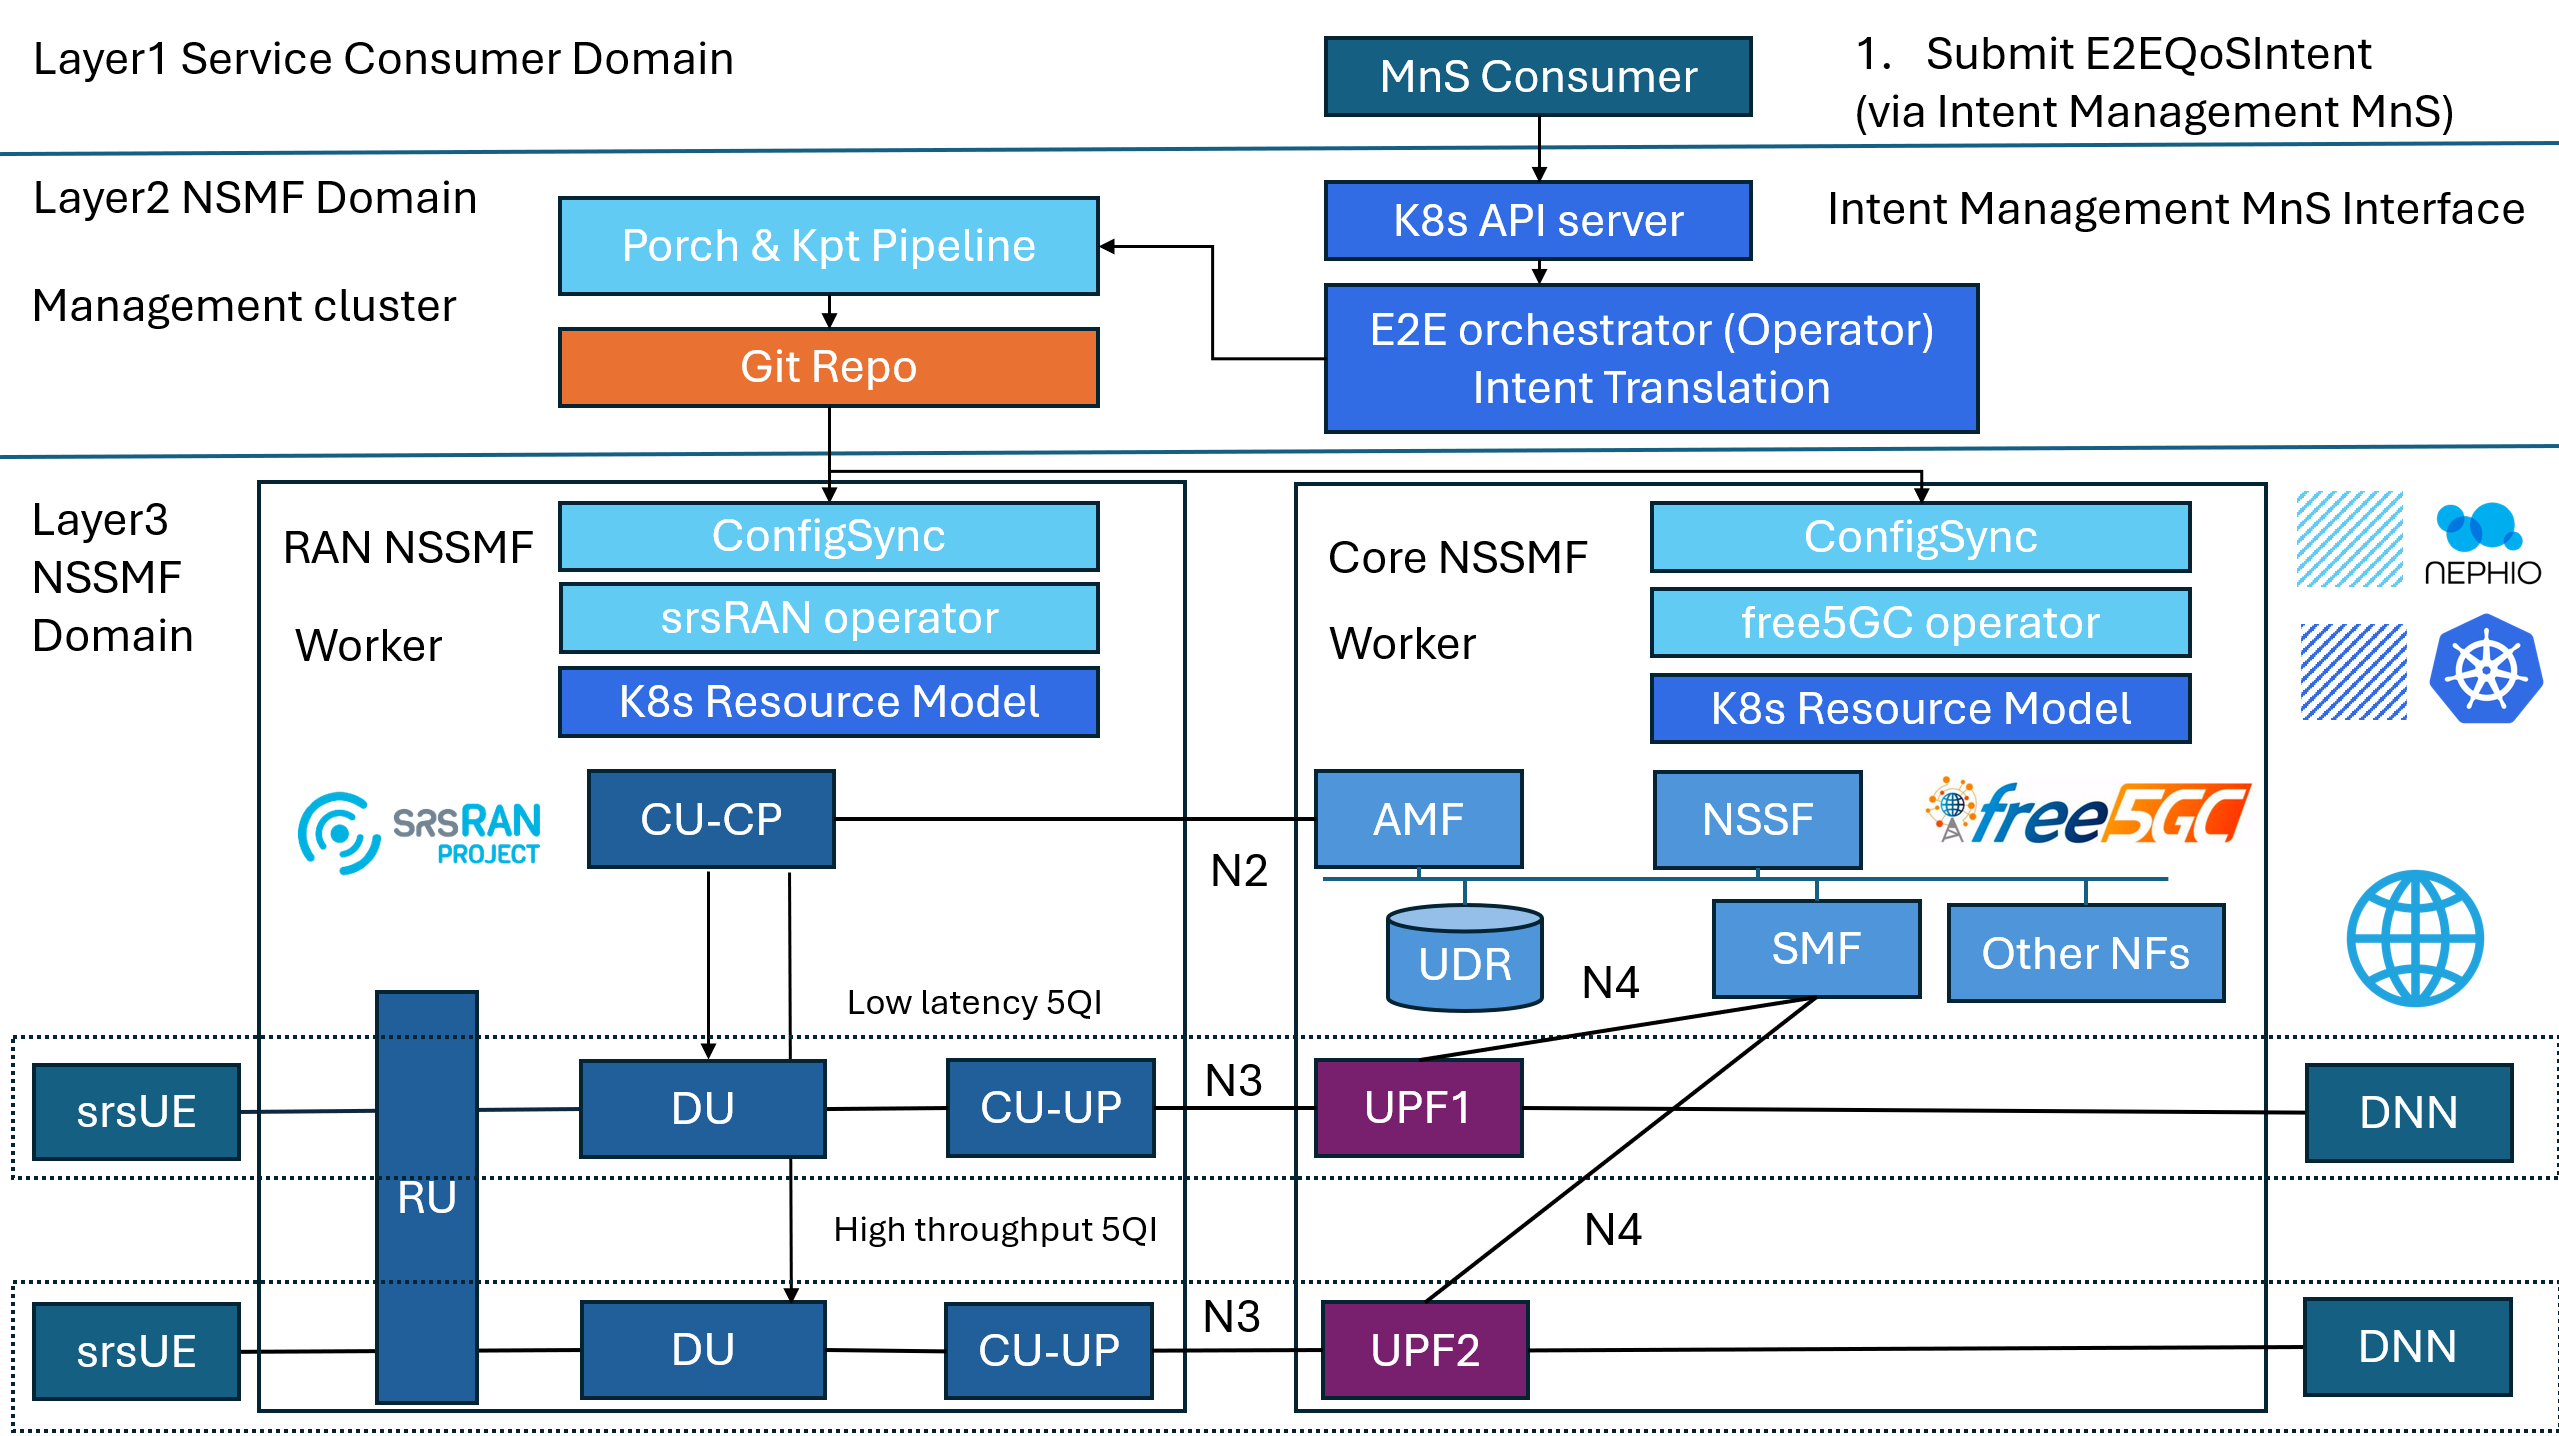
\includegraphics[width=\linewidth]{3.1.1-arch.png}
  \caption{Intent-driven orchestration architecture for coordinating service-level slice intents with RAN and core-domain configuration.}
  \Description{A layered architecture with service consumer, E2E orchestrator, southbound interfaces, and domain execution components for OCUDU, free5GC, Nephio, GitOps, and Kubernetes operators.}
  \label{fig:system_arch}
\end{figure}

Figure~\ref{fig:system_arch} shows the proposed architecture. The system is divided into four logical layers.

\textbf{Service consumer layer.} A consumer submits slice objectives to the Kubernetes API as \texttt{E2EQoSIntent} objects. The API server becomes the intent management interface. This choice avoids a separate northbound REST schema and allows all intent instances to inherit Kubernetes access control, versioning, and event semantics.

\textbf{Intent orchestration layer.} The E2E orchestrator acts as an NSMF and intent handler. It watches intent resources, validates the requested service classes, translates the expectations into domain parameters, and records fulfillment state in the intent status. The orchestrator is implemented as a Kubernetes controller so that failed or partial operations can be retried through reconciliation.

\textbf{Southbound interface layer.} The RAN and core domains are configured through different mechanisms. For RAN, the orchestrator uses Nephio Porch to copy, mutate, propose, and approve a package revision. The approved package is synchronized to the workload cluster by Config Sync. For the core, the orchestrator configures free5GC slice and QoS state through core-domain configuration logic. This hybrid design reflects the maturity of the available open-source components: RAN cell configuration maps naturally to a KRM package, while free5GC subscriber/QoS configuration still requires API- or database-facing integration.

\textbf{Domain execution layer.} The workload cluster runs domain operators. The OCUDU operator consumes KRM resources such as cell and PLMN configuration and renders the final gNB configuration. The free5GC-side logic configures the subscriber and QoS information needed for the intended slices. Both domains report status back to the orchestrator.

\subsection{Intent Model}

Listing~\ref{lst:input_intent} illustrates the intent interface. One resource can contain multiple intent groups so that related slices can be reconciled together. Each group contains context, such as target UEs, and expectations, such as slice type, latency, bandwidth, and resource sharing.

\begin{lstlisting}[caption={Example \texttt{E2EQoSIntent} submitted by a consumer.}, label={lst:input_intent}]
apiVersion: e2e.intent.domain/v1alpha1
kind: E2EQoSIntent
metadata:
  name: slices-intent
spec:
  intentGroups:
    - id: embb
      contexts:
        targetUEs: ["208930000000001"]
      expectations:
        sliceType: eMBB
        bandwidth: high
        resourceShare: Partial
    - id: urllc
      contexts:
        targetUEs: ["208930000000002"]
      expectations:
        sliceType: URLLC
        latency: ultra-low
        resourceShare: Full
\end{lstlisting}

The model intentionally separates \emph{what} the consumer wants from \emph{how} each domain realizes it. For example, \texttt{latency: ultra-low} does not name a scheduler parameter. Instead, it signals that the orchestrator should select a low-latency 5QI and a high-priority RAN slice configuration.

\subsection{Cross-Domain Translation}
\label{subsec:translation}

The translation engine maps intent expectations to concrete domain parameters. Table~\ref{tab:translation} summarizes the mappings used in the prototype. The exact values are policy choices rather than universal constants; the contribution is the translation structure and the ability to materialize it across free5GC and OCUDU.

\begin{table}[t]
  \caption{Intent-to-configuration mapping used by the prototype.}
  \label{tab:translation}
  \begin{tabular}{llll}
    \toprule
    Intent & Core QoS & RAN policy & Priority \\
    \midrule
    eMBB, high bandwidth & 5QI 9 & PRB max 50\% & 10 \\
    URLLC, ultra-low latency & 5QI 85 & PRB max 100\% & 200 \\
    \bottomrule
  \end{tabular}
\end{table}

The core mapping selects 5QI and QFI values for QoS flows. The RAN mapping selects the S-NSSAI and scheduler configuration used by OCUDU. A \texttt{Full} resource-share intent allows the URLLC slice to use up to all available PRBs when needed, while a \texttt{Partial} resource-share intent bounds the eMBB slice to preserve headroom for higher-priority traffic. The RAN priority value reinforces this differentiation when both slices are active.

\subsection{End-to-End Workflow}
\label{subsec:e2e_workflow}

The complete workflow has five stages. First, the orchestrator admits the intent by checking whether the requested slice classes and expectation fields are supported by the current policy table. Second, it translates the accepted intent into domain parameters. The output is deterministic for a given policy table, so an operator can inspect the status field and see which 5QI, QFI, SD, PRB ratio, and priority values were derived from the original request. Third, the RAN parameters are inserted into a Nephio package revision that is proposed and approved for GitOps delivery. Fourth, the core parameters are applied to free5GC subscriber and QoS configuration. Finally, the orchestrator observes domain status and updates the top-level fulfillment state.

This workflow separates intent handling from low-level deployment mechanics. A domain-specific failure does not require the consumer to understand Porch, Config Sync, free5GC subscriber records, or OCUDU ConfigMaps. Instead, the consumer sees a single status surface.

\subsection{Fulfillment and Status}

The orchestrator writes translated parameters and domain status into the CRD status field. This follows the Kubernetes convention that \texttt{spec} is desired state and \texttt{status} is observed state. A typical fulfillment record includes the translated core and RAN parameters, the observed generation, and per-domain states such as \texttt{CONFIGURED}, \texttt{DEGRADED}, or \texttt{FAILED}. This status path is important because intent-driven management requires not only execution but also a machine-readable statement of whether the requested outcome is fulfilled.

\begin{lstlisting}[caption={Representative intent status after translation and domain observation.}, label={lst:intent_status}]
status:
  observedGeneration: 3
  fulfillmentState: FULFILLED
  intentGroupStatuses:
    - id: embb
      core: {fiveQI: 9, qfi: 9, state: CONFIGURED}
      ran:
        sst: 1
        sd: 66051
        maxPrbPolicyRatio: 50
        priority: 10
        state: CONFIGURED
    - id: urllc
      core: {fiveQI: 85, qfi: 85, state: CONFIGURED}
      ran:
        sst: 1
        sd: 1122867
        maxPrbPolicyRatio: 100
        priority: 200
        state: CONFIGURED
\end{lstlisting}

Listing~\ref{lst:intent_status} also provides a practical debugging interface. If the RAN package is synchronized but the core path fails, the two domain states diverge and the top-level fulfillment state can move to \texttt{DEGRADED}. If translation itself fails, no southbound mutation is attempted.

\section{Implementation}
\label{sec:implementation}

The prototype uses three Kubernetes controllers: the E2E Intent Orchestrator, the OCUDU Operator, and Nephio's free5GC Operator. The orchestrator translates \texttt{E2EQoSIntent} resources and coordinates the southbound paths. The two domain operators reconcile the RAN and core workloads as RAN NSSMF and Core NSSMF/VNFM components.

\subsection{Controller Lifecycle}

The controller follows the standard Kubernetes reconciliation pattern. When an \texttt{E2EQoSIntent} is created or updated, the reconciler fetches the current object, checks its generation, computes the desired translated state, and compares it with the last observed status. If the status already matches the current generation, the reconciliation ends without repeating southbound operations. Otherwise, the reconciler runs translation and domain realization and then writes a new status update.

This idempotent structure is important for GitOps integration. Porch and Config Sync may introduce asynchronous delay, and the Kubernetes API may deliver repeated events for the same resource version. The orchestrator therefore treats every reconciliation as a convergence attempt rather than a one-shot command. A failed stage records a reason and is retried according to the controller runtime backoff policy.

\begin{table}[t]
  \caption{Controller stages and observable artifacts}
  \label{tab:controller_stages}
  \begin{tabular}{lll}
    \toprule
    Stage & Main action & Observable artifact \\
    \midrule
    Admit & Check policy table & Status condition \\
    Translate & Derive core/RAN tuple & Intent status \\
    Mutate RAN & Patch KRM package & PackageRevision \\
    Configure core & Bind UE QoS data & Subscriber profile \\
    Observe & Read domain state & Fulfillment state \\
    \bottomrule
  \end{tabular}
\end{table}

Table~\ref{tab:controller_stages} summarizes the reconciliation pipeline. The implementation keeps these stages explicit in code rather than hiding them behind one monolithic handler. This helped testing because each stage can be exercised with a small fixture: an unsupported intent for admission, a known eMBB/URLLC input for translation, a package containing a cell configuration for RAN mutation, and a subscriber record for the core path. The same stage boundaries are also reflected in log messages and status reasons, which makes a failed run easier to inspect from \texttt{kubectl}.

\subsection{RAN Package Mutation}

For the RAN path, the orchestrator uses Nephio Porch as the package control point. The workflow has four steps. First, the orchestrator copies the blueprint package and pulls a mutable package revision. Second, it patches the structured KRM resource that represents OCUDU cell configuration. Third, it pushes and proposes the package revision. Fourth, it approves the package so that the GitOps pipeline can synchronize it to the workload cluster.

Listing~\ref{lst:ran_mutation} shows the resulting RAN slice configuration. The eMBB slice uses SD \texttt{0x010203}, a maximum PRB policy ratio of 50, and priority 10. The URLLC slice uses SD \texttt{0x112233}, a maximum PRB policy ratio of 100, and priority 200.

\begin{lstlisting}[caption={Mutated OCUDU slice configuration generated from intent translation}, label={lst:ran_mutation}]
spec:
  slicing:
    - sst: 1
      sd: 66051
      schedCfg:
        minPrbPolicyRatio: 0
        maxPrbPolicyRatio: 50
        priority: 10
    - sst: 1
      sd: 1122867
      schedCfg:
        minPrbPolicyRatio: 0
        maxPrbPolicyRatio: 100
        priority: 200
\end{lstlisting}

After synchronization, the OCUDU Operator renders the final \texttt{gnb-config.yml} and updates the gNB-related Kubernetes objects. Nephio and Config Sync deliver the KRM objects, and the operator performs the domain-specific realization needed to make that desired state executable by OCUDU. This preserves Git as the source of truth and allows package-level review or rollback.

\begin{figure}[t]
  \centering
  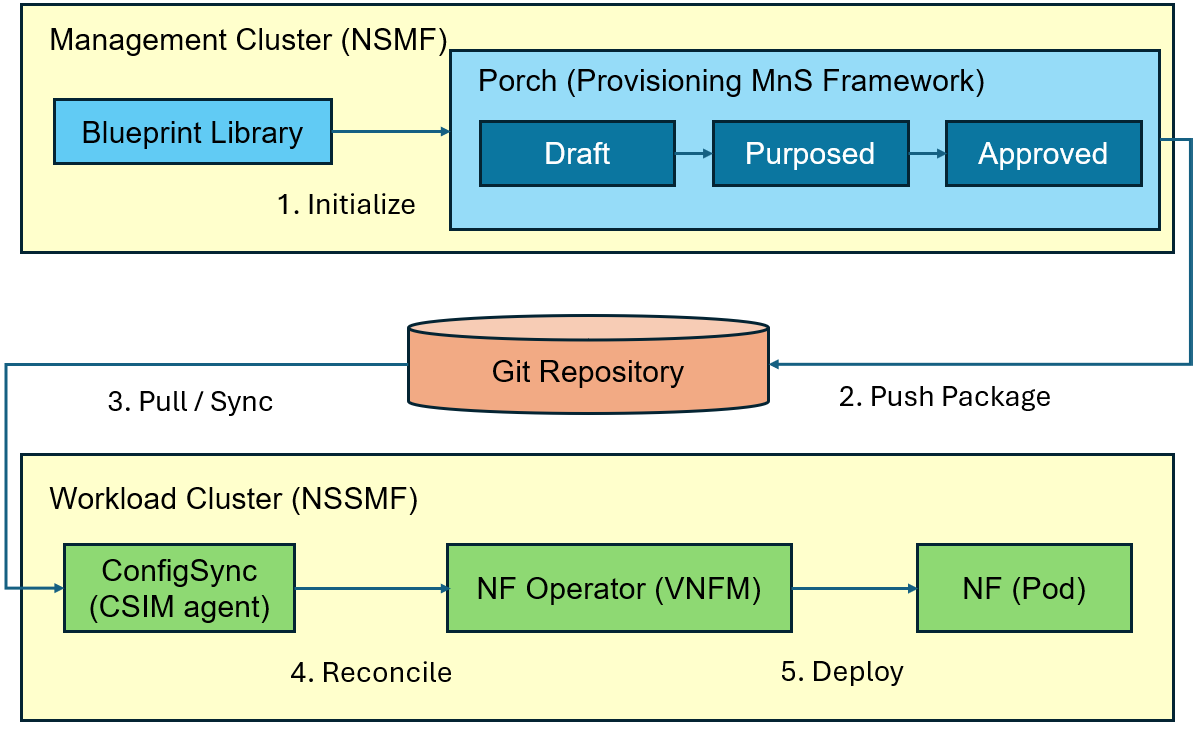
\includegraphics[width=\linewidth]{2.2.3-nephio-workflow-new.png}
  \caption{Nephio-style package workflow used by the RAN orchestration path}
  \Description{A package workflow from management cluster package mutation through Git synchronization to workload cluster application.}
  \label{fig:nephio_workflow}
\end{figure}

Figure~\ref{fig:nephio_workflow} illustrates why the RAN path is modeled as package mutation rather than direct pod modification. The package revision becomes the reviewable artifact, while the workload cluster only consumes approved state. This provides a clean operational boundary: the intent controller decides what RAN policy should change, and the GitOps pipeline decides when the approved configuration reaches the target cluster.

The mutation logic operates on structured YAML objects instead of template strings. The orchestrator locates the cell configuration resource, replaces only the \texttt{spec.slicing} entries, and preserves unrelated physical-layer fields such as band, ARFCN, bandwidth, and subcarrier spacing. It also updates the PLMN slice list so that the broadcast network identity remains consistent with the scheduler configuration. This is a small but important engineering detail: a scheduler entry alone is insufficient if UEs cannot discover or request the same S-NSSAI during registration and session establishment.

The resulting package is intentionally self-contained. A reviewer can inspect the package revision and see the old and new slice entries before approval, while the workload cluster receives the same artifact through Config Sync. This differs from a direct imperative update to a running ConfigMap, where the final state may be correct but the path that produced it is harder to audit or roll back.

\subsection{free5GC Operator and Core-Domain Configuration}

The Core NSSMF path uses the official free5GC Operator provided by Nephio. It watches \texttt{NFDeployment} resources, runs a reconciliation loop, and maintains the desired deployment state of free5GC network functions. This gives the core domain the same Kubernetes-native lifecycle behavior used by other Nephio-managed workloads.

Dynamic subscriber and QoS state follows a complementary path because it is not fully represented by the operator's deployment resources. The orchestrator uses the free5GC WebConsole API to configure S-NSSAI, subscriber binding, PDU session QoS, QFI, and 5QI for the target UEs. Separating NF deployment from subscriber configuration keeps the Core NSSMF role explicit without attributing unsupported runtime functions to the official operator.

The core implementation performs consistency checks before reporting success. For each target UE, it verifies that the intended S-NSSAI and QoS profile are present in the core-domain state. This does not prove that every packet will receive the desired treatment, because runtime QoS still depends on UPF and kernel behavior, but it does prove that the control-plane configuration requested by the intent is present.

The core path is organized around UE binding. For every \texttt{targetUEs} entry in an intent group, the orchestrator ensures that the subscriber profile contains the intended S-NSSAI and that the session management data contains the selected 5QI/QFI values. If the UE profile already exists, the orchestrator updates only the slice-related fields required by the active intent. If the profile is absent in the testbed, it can create the minimal subscriber state needed for the experiment. This behavior makes repeated experiments reproducible because the same intent converges to the same core-domain state.

The implementation treats this path as a compatibility layer rather than a permanent architectural preference. A fully declarative core package would be cleaner because RAN and core changes could share the same package lifecycle. However, forcing all free5GC subscriber data into an incomplete package abstraction would make the prototype less reliable. The hybrid path therefore preserves the most important property for this paper: a single high-level intent produces aligned core and RAN configuration, even though the two domains currently require different delivery mechanisms.

\subsection{OCUDU Operator and Hierarchical RAN Resources}

\texttt{OCUDUConfig} captures application-level settings such as CU/DU deployment and radio-emulation parameters. \texttt{OCUDUCellConfig} captures cell-level settings, including slice-aware scheduling. \texttt{PLMNConfig} captures network identity and S-NSSAI information. Splitting the configuration this way avoids large monolithic resources and lets the operator validate each layer independently before producing the final ConfigMap.

The OCUDU Operator performs reference walking across these resources. Starting from the deployment resource, it resolves the referenced application, cell, and PLMN objects, validates that the referenced slices are mutually consistent, and then renders the final gNB configuration. When rendering succeeds, it updates Kubernetes resources and marks the deployment as ready. When a referenced object is missing or inconsistent, it records a condition instead of producing a partial configuration. This local check is separate from the E2E orchestrator's admission policy and protects the workload cluster from broken package content.

\begin{lstlisting}[caption={Representative rendered scheduler fragment}, label={lst:rendered_scheduler}]
cell_cfg:
  slicing:
    - sst: 1
      sd: 0x010203
      sched_cfg:
        min_prb_policy_ratio: 0
        max_prb_policy_ratio: 50
        priority: 10
    - sst: 1
      sd: 0x112233
      sched_cfg:
        min_prb_policy_ratio: 0
        max_prb_policy_ratio: 100
        priority: 200
\end{lstlisting}

Listing~\ref{lst:rendered_scheduler} shows the final form consumed by the RAN software. Comparing this artifact with the original intent and the intermediate package gives a concrete end-to-end trace: service expectation, translated profile, KRM package, and rendered runtime configuration.

\subsection{Failure Handling}

The prototype distinguishes three failure classes. Translation failures occur before any southbound operation, such as an unsupported slice type or an impossible combination of expectations. Delivery failures occur when a package cannot be mutated, approved, or synchronized. Domain failures occur when either domain operator cannot reconcile its delivered resources. These classes are written into intent status so that the consumer can tell whether the problem is semantic, pipeline-related, or domain-local.

This failure taxonomy is deliberately aligned with future 3GPP intent features. Feasibility checks and conflict reports can be added before translation, while negotiation and utility functions can be added as policy modules that select among alternative translations. The current implementation is therefore a first step toward richer intent handling rather than a closed one-off script.

\section{Evaluation}
\label{sec:evaluation}

The evaluation asks three questions:
\begin{enumerate}
  \item Can the system materialize an intent into consistent core and RAN slice configuration?
  \item Does the generated RAN configuration differentiate eMBB and URLLC traffic?
  \item Where is orchestration time spent in the management path?
\end{enumerate}

\subsection{Testbed}

The testbed uses MicroK8s v1.28, Nephio R5, free5GC v4.2.1, OCUDU release 26.04, and an srsUE-based emulation environment. The management and workload clusters run in a virtualized environment with 10 vCPUs and 32 GB of memory. A separate local environment is used to validate the data-plane behavior of the generated OCUDU configuration. Traffic measurements use \texttt{iperf3} UDP flows~\cite{iperf3_manual}.

\begin{table}[t]
  \caption{Software components used in the prototype.}
  \label{tab:software}
  \begin{tabular}{ll}
    \toprule
    Component & Version \\
    \midrule
    Kubernetes distribution & MicroK8s v1.28 \\
    Package orchestration & Nephio R5 \\
    5G core & free5GC v4.2.1 \\
    RAN & OCUDU release 26.04 \\
    UE emulator & srsUE v25.10 \\
    Orchestrator & Golang/Kubebuilder prototype \\
    \bottomrule
  \end{tabular}
\end{table}

The evaluation uses two deployment modes because they answer different questions. The local mode removes Kubernetes and GitOps from the data path and establishes whether the generated RAN scheduling configuration has the intended qualitative effect. The cloud-native mode then verifies whether the same configuration can be produced through the proposed intent, Nephio, and operator pipeline. This separation is useful because a negative result in the cloud-native test could come from either an incorrect slice policy or from the deployment pipeline; the local baseline helps separate those causes.

The management cluster hosts the E2E orchestrator and Porch-facing package workflow. The workload cluster hosts free5GC, the OCUDU-related resources, Config Sync, and the domain operator. UE and traffic-generation components are treated as test resources rather than managed network functions. This keeps the system under test focused on the infrastructure that would normally be operated by an NSMF/NSSMF-style automation stack.

\subsection{Metrics}

The evaluation separates data-plane and management-plane metrics. The data-plane measurements focus on throughput, packet loss, and jitter as reported by \texttt{iperf3}. These metrics are not intended to certify carrier-grade QoS; they are used to confirm whether the RAN scheduler reacts to the generated slice parameters. The management-plane measurements focus on orchestration latency and fulfillment state. This distinction is important because an intent system can correctly configure the network but still be too slow for a particular operational use case.

For management-plane latency, the most relevant question is not only total time but also the distribution across stages. A long delay inside the orchestrator would suggest inefficient translation or API use. A long delay inside GitOps synchronization suggests a trade-off between auditability and actuation speed. A long delay inside the local operator would indicate domain-specific rendering or rollout overhead.

\begin{table}[t]
  \caption{Traffic model for data-plane experiments.}
  \label{tab:traffic_model}
  \begin{tabular}{llll}
    \toprule
    Phase & Time & Active flows & Purpose \\
    \midrule
    1 & 0--15 s & eMBB & Baseline throughput \\
    2 & 15--45 s & eMBB + URLLC & Resource competition \\
    3 & 45--60 s & eMBB & Recovery behavior \\
    \bottomrule
  \end{tabular}
\end{table}

Table~\ref{tab:traffic_model} defines the common traffic pattern. The overlap phase is the key interval because it creates contention between a throughput-oriented slice and a latency-sensitive slice. A correct configuration should not necessarily maximize total throughput in this interval; it should shift resource allocation toward the URLLC profile because the input intent gives that profile higher priority and a full PRB policy bound.

\subsection{Data-Plane Slice Differentiation}

The first experiment validates the generated slice configuration in a local environment. Two UEs are associated with different slices. UE1 is mapped to eMBB with 5QI 9 and a partial PRB share. UE2 is mapped to URLLC with a delay-critical 5QI and a full PRB share. The traffic pattern has three phases: only eMBB is active from 0--15 seconds, both eMBB and URLLC are active from 15--45 seconds, and only eMBB remains active from 45--60 seconds.

\begin{figure}[t]
  \centering
  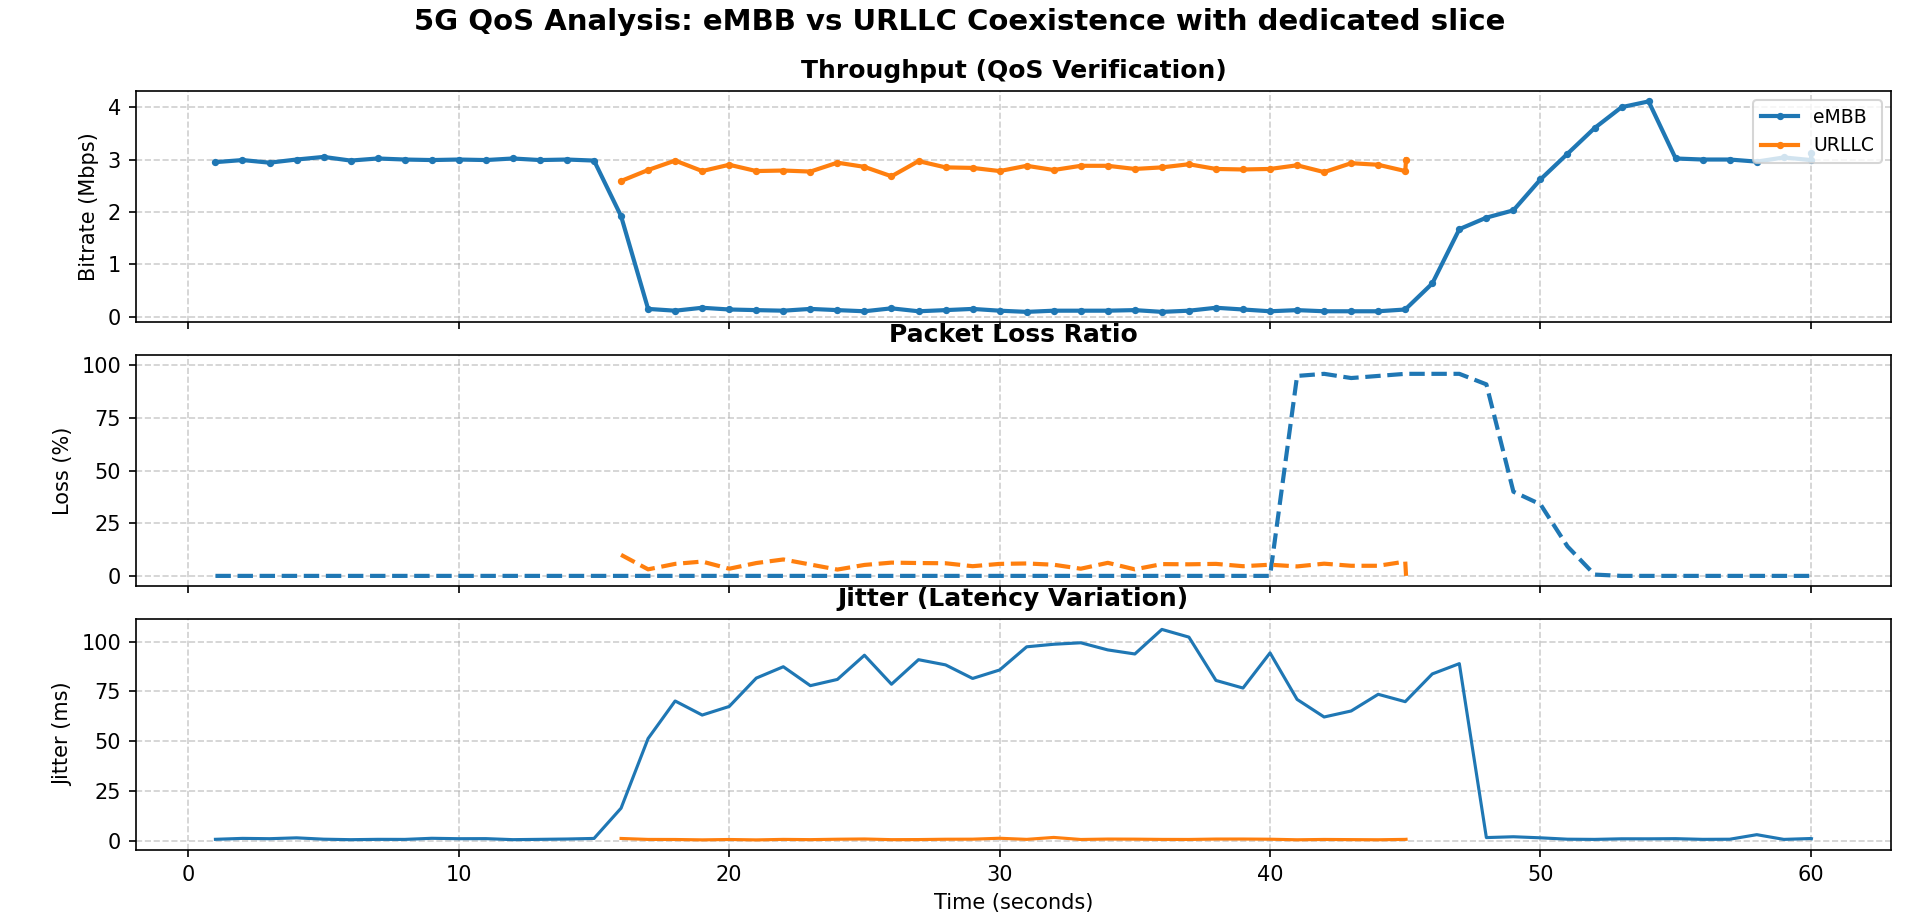
\includegraphics[width=\linewidth]{4.2.1-urllc-vs-embb.png}
  \caption{Local eMBB and URLLC traffic behavior under the generated slice scheduling configuration.}
  \Description{A time-series plot comparing eMBB and URLLC traffic across three phases. URLLC receives higher priority while both flows are active, and eMBB recovers after URLLC stops.}
  \label{fig:local_qos}
\end{figure}

Figure~\ref{fig:local_qos} shows that the RAN scheduler reacts to the generated PRB and priority configuration. During the overlap period, URLLC traffic obtains preferential treatment and eMBB throughput is reduced. After the URLLC flow stops, eMBB recovers. This result does not claim strict end-to-end URLLC guarantees; rather, it confirms that the intent-generated OCUDU configuration reaches the scheduler and produces the expected qualitative behavior.

The local result also exposes a practical limitation of software RAN experiments. Because all components run on general-purpose hosts, buffering and CPU scheduling can affect observed loss and jitter. We therefore interpret the result as evidence of relative slice differentiation. The key observation is that the change in active slice mix leads to the expected change in traffic allocation.

The eMBB degradation during the overlap phase is not instantaneous. In several runs, throughput and loss change after a short delay because buffers absorb transient congestion before packet drops become visible to \texttt{iperf3}. This behavior is expected in a software stack where queueing occurs at multiple layers. The important point is the phase relationship: degradation appears only after the competing URLLC flow begins, and recovery appears after that flow ends. This phase relationship supports the claim that the generated scheduler policy, rather than background load, is responsible for the observed differentiation.

\subsection{Kubernetes/Nephio Deployment}

The second experiment runs the orchestration path through the Kubernetes and Nephio environment. The same eMBB and URLLC intent is submitted as a CRD. The orchestrator mutates the RAN package, Config Sync applies the package to the workload cluster, and the OCUDU operator renders the final configuration.

\begin{figure}[t]
  \centering
  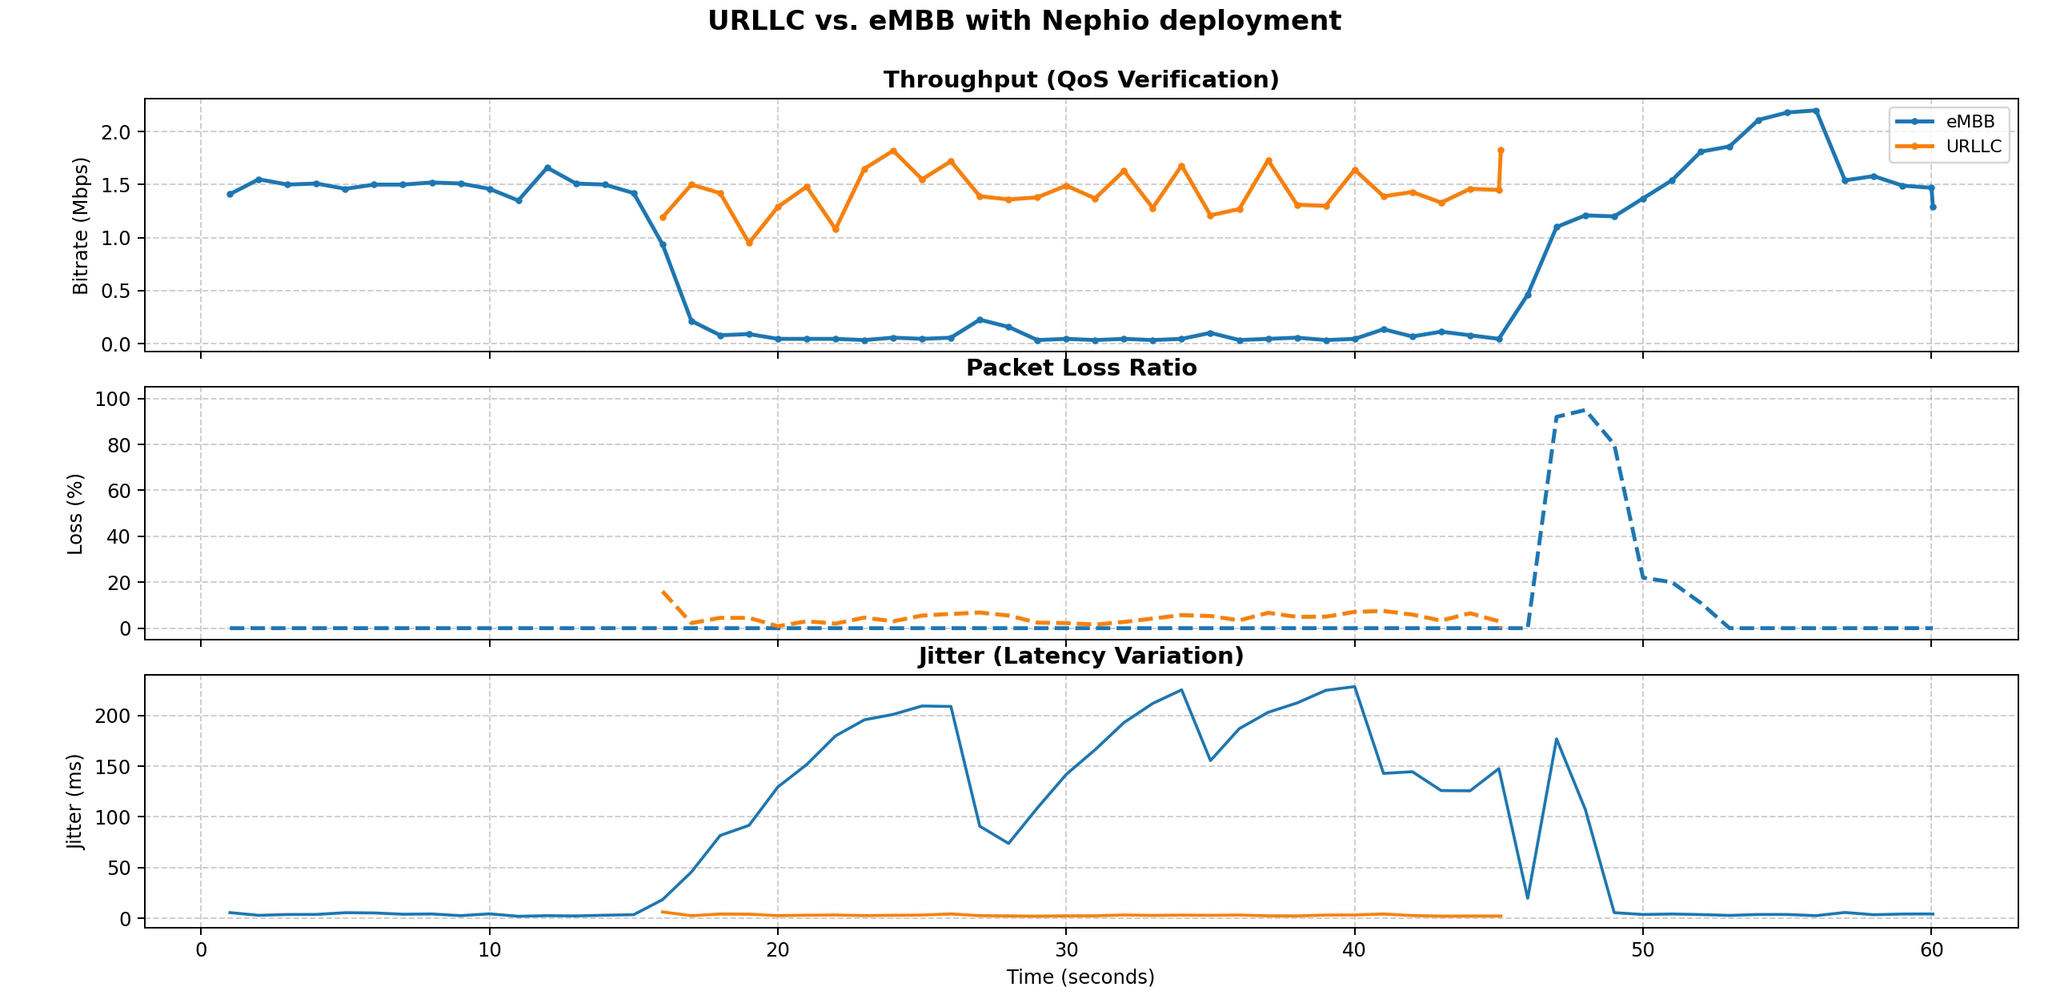
\includegraphics[width=\linewidth]{4.2.2-urllc-vs-embb.png}
  \caption{Slice behavior after orchestration through the Nephio and Kubernetes workflow.}
  \Description{A time-series plot showing that URLLC receives more throughput than eMBB during the overlap period in the Kubernetes-based testbed, though absolute throughput is lower than in the local environment.}
  \label{fig:k8s_qos}
\end{figure}

Figure~\ref{fig:k8s_qos} shows the same differentiation trend after orchestration through the cloud-native workflow. Absolute throughput is lower than in the local test because the virtualized Kubernetes environment adds scheduling and networking overhead. Nevertheless, the generated configuration remains effective: when URLLC becomes active, it receives a larger share of available radio resources, and eMBB throughput decreases accordingly.

The cloud-native experiment also validates configuration consistency across asynchronous control loops. The E2E orchestrator completes its mutation before Config Sync necessarily applies the package; the domain operator then runs after the package reaches the workload cluster. A correct final result therefore requires all three loops to converge on the same desired state. The observed traffic behavior provides data-plane evidence of this convergence, while the fulfillment checks in the next subsection provide management-plane evidence.

In the Kubernetes testbed, the maximum stable offered rate is lower than in the local baseline. This result is not surprising because the experiment runs the 5G core, RAN components, UE emulation, and automation services inside a virtualized cluster. The measured absolute rate should therefore be read as a property of the testbed, not as a limit of the intent design. The comparison that matters for this paper is whether the relative eMBB/URLLC behavior is preserved when the configuration is generated and delivered through the full orchestration path.

\subsection{Fulfillment Verification}

After each orchestration run, we verify fulfillment at three levels. First, the intent status must contain the translated parameters for each intent group. Second, the RAN package in the workload cluster must contain the intended S-NSSAI, PRB ratio, and priority. Third, the generated OCUDU ConfigMap must contain the corresponding scheduler configuration. Table~\ref{tab:verification} summarizes these checks.

\begin{table}[t]
  \caption{Fulfillment checks after applying the two-slice intent.}
  \label{tab:verification}
  \begin{tabular}{lll}
    \toprule
    Layer & Artifact & Expected result \\
    \midrule
    Intent API & \texttt{E2EQoSIntent.status} & \texttt{FULFILLED} \\
    RAN package & \texttt{OCUDUCellConfig} & Two S-NSSAIs \\
    RAN runtime & gNB ConfigMap & PRB/priority rendered \\
    Core domain & UE QoS profile & 5QI/QFI configured \\
    \bottomrule
  \end{tabular}
\end{table}

These checks are intentionally simple and reproducible. They give the operator confidence that the declarative request, package artifact, and runtime configuration are aligned. They also make it easier to localize faults: for example, if the package is correct but the ConfigMap is not, the likely issue is in the domain operator rather than the translation engine.

The verification script performs these checks after each run rather than relying only on the final traffic plot. This matters because data-plane results can be noisy in an emulated setup. A noisy result with correct fulfillment indicates a testbed performance issue, while a noisy result with incorrect fulfillment indicates an orchestration bug. In our runs, the translated intent status, package resource, rendered ConfigMap, and core profile agreed on the selected S-NSSAIs and QoS values.

\subsection{Management-Plane Latency}

We measure orchestration latency by recording four timestamps: $T_0$, when the \texttt{E2EQoSIntent} is applied; $T_1$, when Porch package mutation and approval complete; $T_2$, when Config Sync applies the package to the workload cluster; and $T_3$, when the OCUDU operator updates the final ConfigMap. The total latency is:
\begin{equation}
  T_{total} = (T_1 - T_0) + (T_2 - T_1) + (T_3 - T_2).
\end{equation}

\begin{figure}[t]
  \centering
  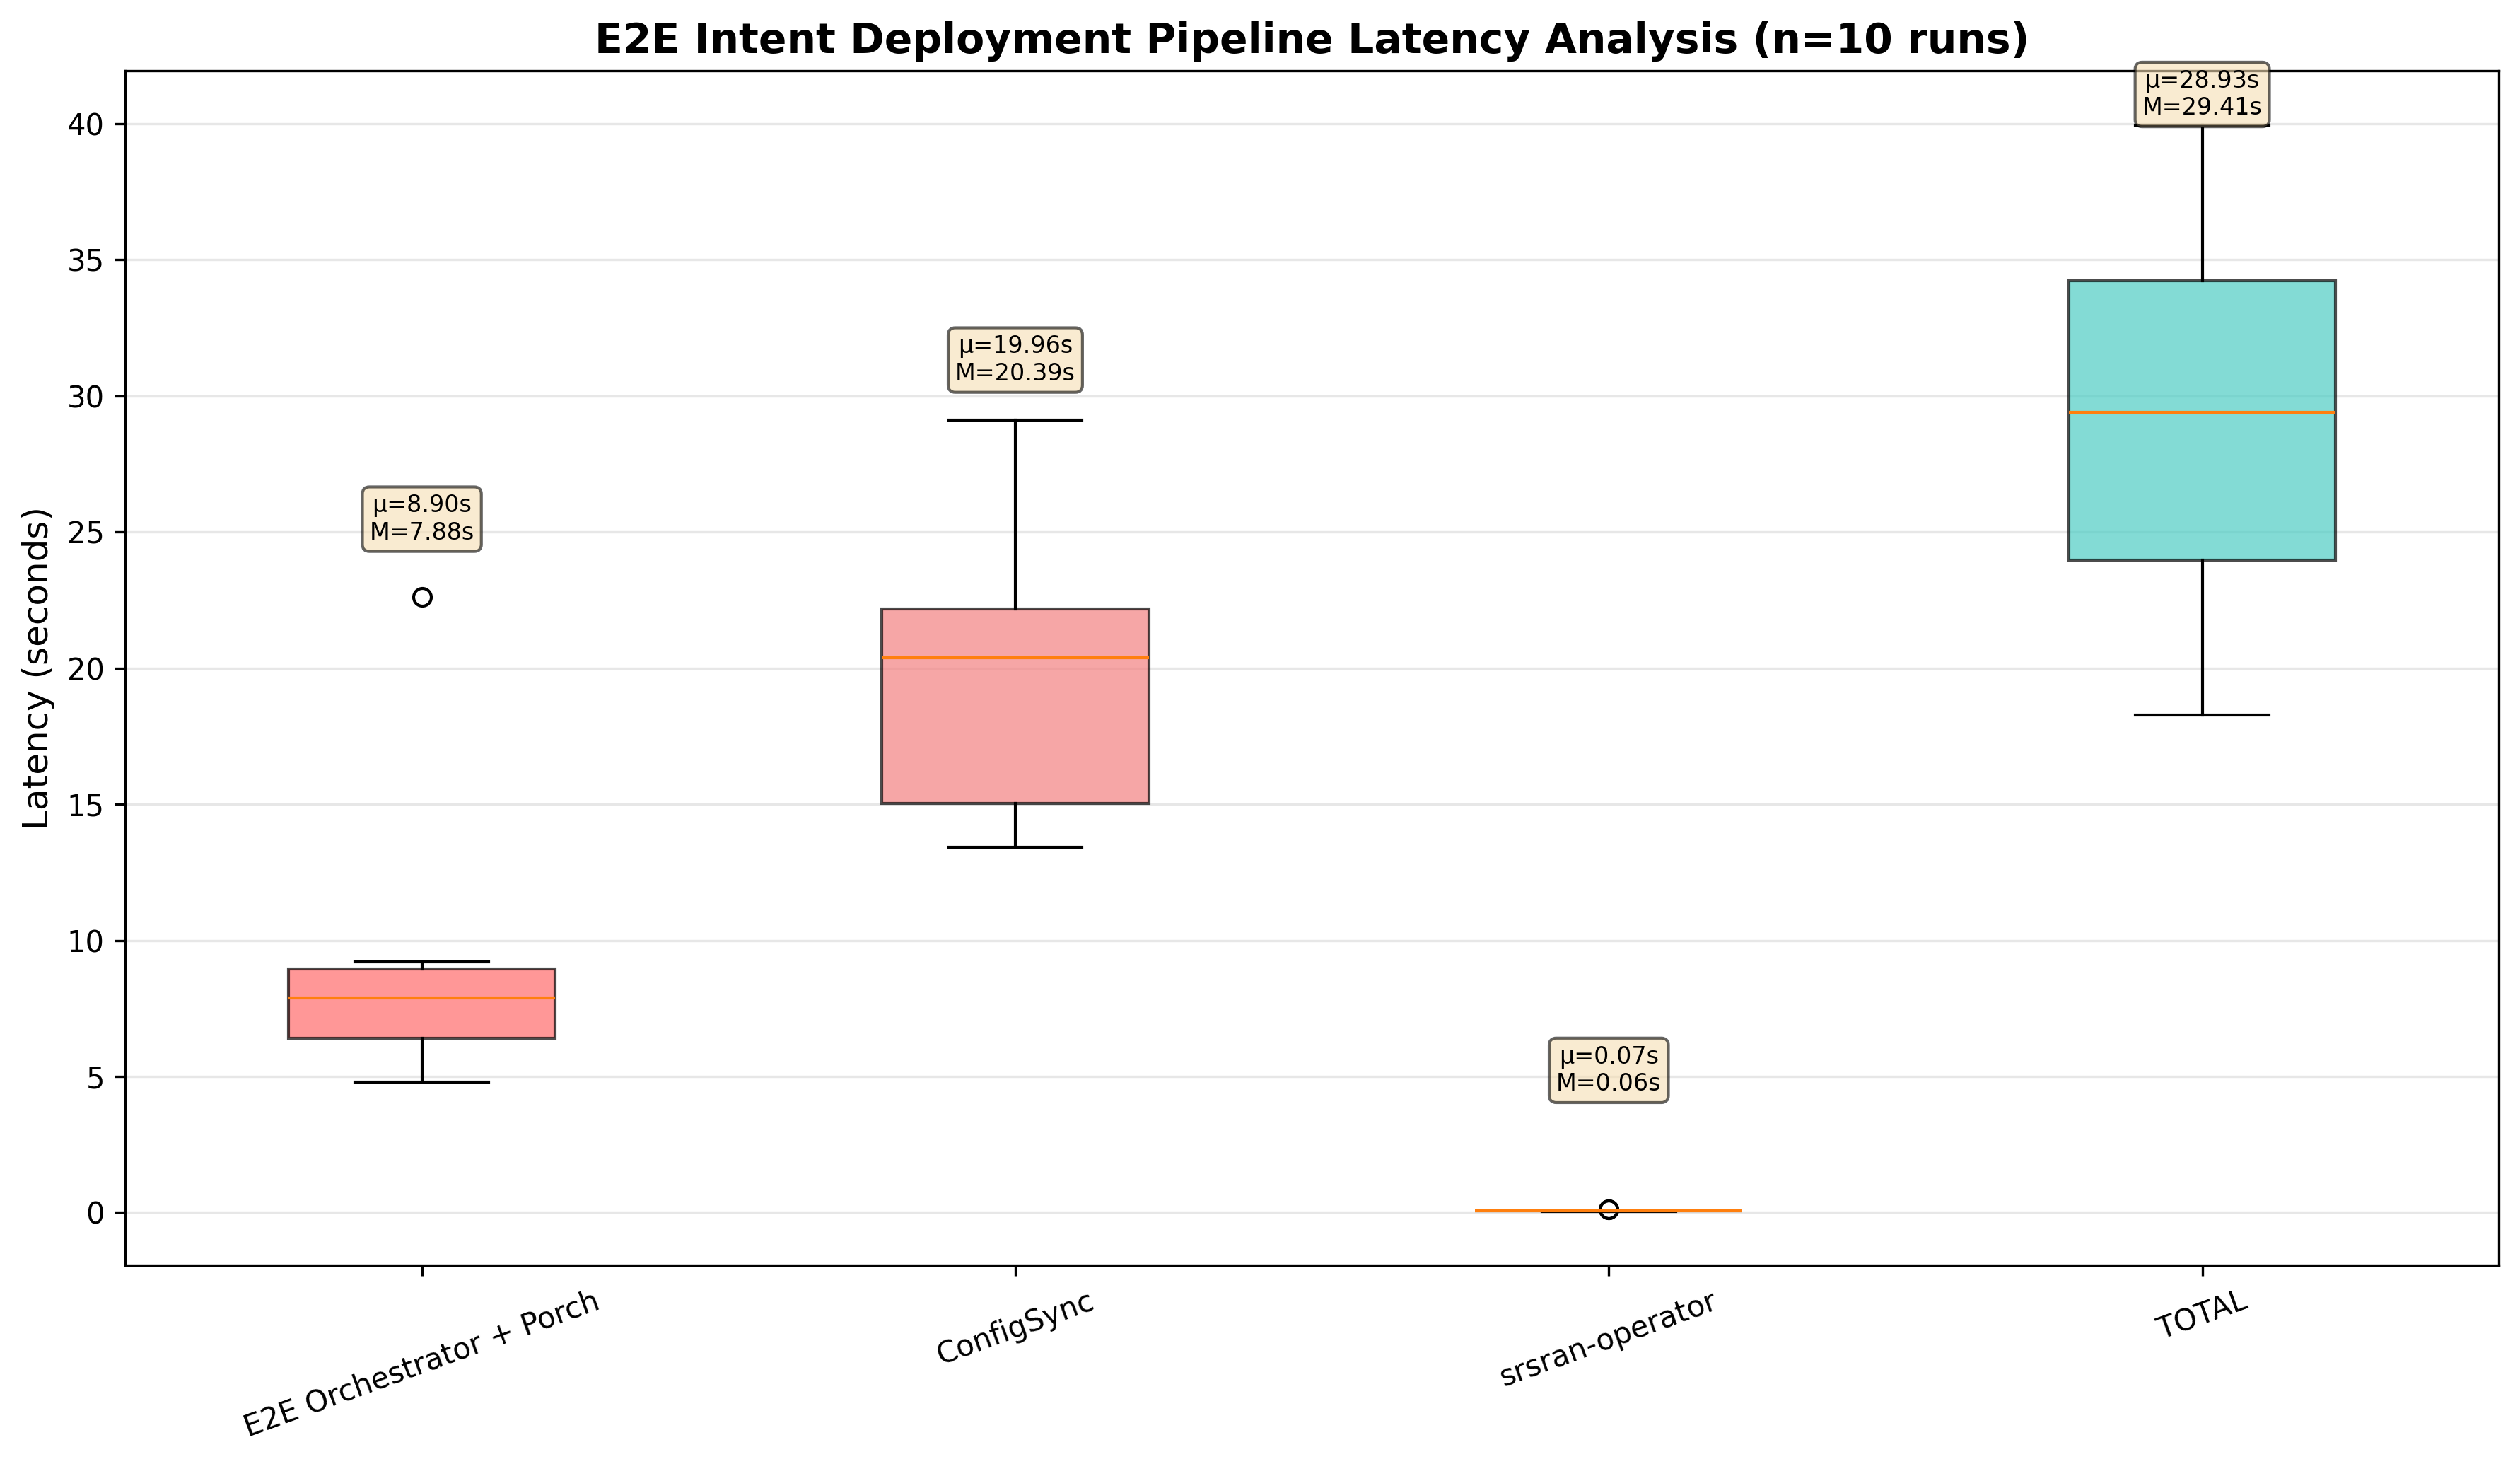
\includegraphics[width=\linewidth]{4.3.2-latency.png}
  \caption{Management-plane latency distribution across orchestration stages.}
  \Description{A latency plot showing that GitOps synchronization dominates total orchestration time, while operator reconciliation is short.}
  \label{fig:latency}
\end{figure}

\begin{table}[t]
  \caption{Representative orchestration latency sample.}
  \label{tab:latency}
  \begin{tabular}{lr}
    \toprule
    Stage & Time \\
    \midrule
    Orchestrator + Porch, $T_1 - T_0$ & 7.348 s \\
    Config Sync, $T_2 - T_1$ & 22.659 s \\
    OCUDU operator, $T_3 - T_2$ & 0.068 s \\
    \midrule
    Total, $T_{total}$ & 30.077 s \\
    \bottomrule
  \end{tabular}
\end{table}

Figure~\ref{fig:latency} and Table~\ref{tab:latency} show that total orchestration latency is about 30 seconds in the representative run. The dominant component is GitOps synchronization, not local operator reconciliation. This is an important engineering trade-off: GitOps adds auditability and rollback, but it is not a sub-second control loop. The design is therefore suitable for slice provisioning and policy updates, while fast per-packet or per-TTI adaptation should remain inside the RAN scheduler or a near-real-time control loop.

The result also gives guidance for future optimization. The orchestrator and Porch stage contains translation, package mutation, and approval; at roughly seven seconds in the representative sample, it is visible but not dominant. The local operator stage is effectively negligible in comparison, which suggests that rendering a cell configuration from structured resources is not the bottleneck. Reducing total actuation time would therefore mainly require changing the synchronization policy, shortening the Config Sync interval, or adding a controlled fast path for low-risk updates. Such changes would trade some audit delay for faster convergence and should be exposed as operator policy rather than hidden inside the intent translation logic.

\subsection{Summary of Findings}

The evaluation supports three findings. First, the CRD-based intent interface is sufficient to express multiple slice objectives and preserve their translated parameters in status. Second, the generated OCUDU configuration changes traffic allocation in the expected direction for eMBB and URLLC flows. Third, the orchestration path is dominated by GitOps synchronization time. These findings suggest that the design is appropriate for provisioning and policy-level reconfiguration, but not for millisecond-scale radio adaptation.

\section{Conclusion and Future Work}
\label{sec:conclusion}

This paper presented an intent-driven orchestration system for 5G RAN and core network slices using free5GC, OCUDU, Kubernetes, and Nephio. The E2E orchestrator translates service expectations into aligned core and RAN parameters, while the OCUDU and free5GC Operators provide the RAN NSSMF and Core NSSMF/VNFM reconciliation paths. Dynamic core subscriber state is injected through a complementary free5GC-facing interface. Experiments show the intended eMBB/URLLC traffic differentiation, while the measured operator stage confirms that domain reconciliation is not the dominant source of the approximately 30-second management latency; GitOps synchronization is.

\subsection{Limitations}

The prototype demonstrates a control pattern rather than a production-ready slice-management platform. It focuses on two representative service classes, eMBB and URLLC; a production system would need a richer catalog of service profiles, tenant quotas, authentication and authorization policies, and explicit rules for deciding whether a requested intent can be accepted.

The evaluation uses emulated UEs and a virtualized Kubernetes environment, so the throughput results should not be interpreted as a production performance benchmark. They validate configuration effects rather than the maximum capacity of the underlying RAN or core implementation. CPU scheduling, virtual networking, and buffering can influence measured loss, jitter, and throughput. The most important evidence is therefore relative: when the generated slice configuration changes, traffic allocation changes in the expected direction.

\subsection{Future Work}

Future work should add 3GPP Release 18 and Release 19 style intent features, including fulfillment feasibility checks, conflict reports, negotiation, and quantitative utility functions. An admission controller could reject impossible or conflicting intents before they trigger package mutation. For example, two tenants could request full PRB access for different URLLC slices at the same time; the current prototype can detect unsupported input, but it does not yet negotiate alternatives or compute a utility-based compromise.

The hybrid southbound design should also be refined. RAN configuration and free5GC NF deployment already use Nephio/GitOps and domain operators. Dynamic core subscriber and QoS configuration still uses free5GC-facing logic because that state is not fully represented by the operator's deployment resources. A future implementation should migrate more subscriber state into declarative resources so that both domains can share the same package lifecycle, audit trail, and rollback behavior.

On the data plane, deeper integration with Linux traffic control, UPF-level QoS enforcement, or additional OCUDU scheduling hooks could improve end-to-end differentiation beyond RAN scheduling alone. On the management plane, reducing GitOps synchronization latency or allowing policy-controlled fast paths would make the system applicable to a broader range of operational workflows.


\begin{acks}
This work was conducted in the context of open-source 5G core and RAN experimentation. The authors thank the free5GC, OCUDU, Kubernetes, and Nephio communities for maintaining the software foundations used in this study.
\end{acks}

\balance
\bibliographystyle{ACM-Reference-Format}
\bibliography{refs}

\end{document}
